% Matlab.tex
%
% Notes:
%
% o Rename this file appropriately.
%
% o Complete relevant sections below.
%
% o Use markup commands defined in scirun-doc.sty.
%   Avoid presentation markup (e.g. \textbf or \emph).
%
% o To make your document web-friendly, use commands from html package. See
%   latex2html manual or the book "The Latex Web Companion."
%
% o Don't add new subsections, but freely subsubsection 
%   existing subsections.
%
% o Add local commands if desired (via \newcommand).  But first check for
%   equivalent markup in scirun-doc.sty.
%
% o Only use packages distributed with Latex2e.
%
% o Cite references with the \cite command. Put citations in
%   a bib file and send along with this file.
%
% o Please include at least one image of tk GUI. Provide 
%   an EPS version and a web friendly version (e.g., jpeg or gif).
%
% o Including images:  Create a figure command for each figure using the
%   template below.  Copy the template (make a copy of the template
%   for each figure) and uncomment only the first '%' in each line.
%   Then replace bracketed text with appropriate values.  Here is the
%   template: 

\newcommand{\fgr}[3]
{
\begin{figure}[htb]
\centerline{\epsfig{file=../psfigs/#1.ps,width=#2}}
\caption{\label{fig:#1} #3 }
\end{figure}
}

% 
% {\centerline{\includegraphics{../psfigs/tst1.ps}}}
%%begin{latexonly}
%  \newcommand{\<figure command name>}%
%  {\centerline{\includegraphics[options]{<path to eps file>}}}
%%end{latexonly}
%\begin{htmlonly}
%  \newcommand{\<figure command name (same as above)>}{%
%  \htmladdimg[options]{<path to jpg file>}}
%\end{htmlonly}
%
%   Where in the ``latexonly'' part, ``options'' is a list of key-value pair
%   options.  Typically the options specify graphic width, height, and
%   bounding box.  See ``The Latex Graphics Companion'' for more
%   information.  Note that we are using ``\includegraphics'' command
%   from the ``graphicx'' package.
%
%   In the ``htmlonly'' part ``options'' is a list options such as ``align'',
%   ``width'', ``height'', and ``alt''.  See ``The Latex Web Companion'' for
%   details.
%   
%   Now to actually create figures enclose each figure command as follows:
%
%\begin{figure}
%  \begin{makeimage}
%  \end{makeimage}
%  \<figurecommand>
%  \caption{\label{fig:<figure label>} <Caption text>}
%\end{figure}
%
%   and replace bracket text appropriately.
%   

% Uncomment following 5 commented lines if you want to process this document
% with Latex. You must also uncomment the last line of the file.

\documentclass[notitlepage,11pt]{article}
\usepackage{graphicx}
% \usepackage{html}
\usepackage{epsfig}
\usepackage{scirun-doc}
\begin{document}
%%%%%%%%%%%%%%%%%%%%%%%%%%%%%%%%%%%%%%%%%%%%%%%%%%%%%%%%%%%%%%%%%%%%%%

\ModuleRef{\Module{Matlab}}{\Category{DataIO}}{\Package{MatlabInterface}}

\subsection{Summary} \indent

The MatlabInterface module
enables calls to Matlab scripts within the \sr{} environment.
This is accomplished
by first establishing an independent Matlab process and second,
as SCIRun communicates with that process via network sockets.

Possible uses of the MatlabInterface include both simple tasks
such as converting SCIRun files to Matlab files, and vice-versa.
In addition, the module completes more complex tasks such as creating
interactive \sr{} programs calling to Matlab scripts for real-time applications.

\subsection{Use}

\subsubsection{Concept} \indent

SCIRun communicates with Matlab via network sockets. The communication
overhead is minimized when both packages reside on the same machine,
and may increase (depending on the network speed) if Matlab is
runs at the remote host.

The choice of a network communication model (as opposed to hard-compiling
Matlab codes into \sr{}) is determined by incompatibilities in Matlab
libraries, and by higher flexibility of the communication model.
The network communication model allows both remote calls to Matlab
scripts, and uses Matlab as a scripting engine to process
interactive user requests. This model resolves potential licensing
conflicts, and provides convenience by saving extra installation time
in the situation where SCIRun and Matlab are installed on different hosts.

\subsubsection{Location and Installation} \indent

We assume that the environment variable {\bf \$SCIRun} points to the root
of the SCIRun source tree, and the package executables are compiled in the
directory {\bf \$SCIRun/bin}.

To install MatlabInterface package, at configure time, provide the
following option to the configure script: \\
{\bf configure --with-package=MatlabInterface} \\
and run {\bf gmake } in {\bf \$SCIRun/bin} directory
to compile the package. 

The MatlabInterface {\bf Matlab} module, which provides communications with 
the Matlab engine on the \sr{} side, is located in MatlabInterface 
package under {\bf DataIO}. Matlab engine scripts, as well as test 
example nets (({\bf tst*.net} files) are located in SCIRun source tree: \\
{\bf \$SCIRun/src/Packages/MatlabInterface/matlab/engine }\\

\subsubsection{Examples} \indent

Examples are the best way to learn how to work with MatlabInterface.
There are five examples attached to the package. The first three
examples assume that SCIRun and Matlab reside on the same host.
The fourth example addresses situations where SCIRun and Matlab are
on different hosts. Example five demonstrates
application of the MatlabInterface to call the focusing inversion routine.

There are three example scripts, named {\bf tst1.net, tst2.net and tst3.net}
that have been written for situations where SCIRun and 
Matlab are installed on the same machine. 
We also assume that the user works from under a Linux (or Unix)
shell and the Matlab package may be accessed in the path. 

To run these examples, change your current directory to \\
{\bf cd \$SCIRun/src/Packages/MatlabInterface/matlab/engine } \\
and execute SCIRun with first test net: \\
{\bf \$SCIRun/bin/scirun  tst1.net} \\
The resulting screen appears in Figure \ref{fig:tst1}.

\subsubsection{Example 1: Save Matlab matrix in SCIRun format} \indent

The first test generates a random matrix under Matlab and sends the
results to \sr{}, where the matrix is saved into a \sr{} file. 

Figure \ref{fig:tst1} shows the SCIRun environment window on the top,
and Unix terminal at the bottom, from where the package was started
(window with black background and title ``rapture'' in Figure 
\ref{fig:tst1}).  Certain diagnostic output is directed into Unix 
terminal window. 

The Matlab GUI dialog window (with the title
``Matlab\_O'' in Figure \ref{fig:tst1} is superimposed onto the \sr{}
window. The Matlab commands are entered in the field with the white
background in the Matlab dialog window.
In the first test example (Figure \ref{fig:tst1}
the command is: \\
{\bf o1=rand(5,5);} \\

The host:the port line is on top of the Matlab dialog window that contains the network address (IP or name and port) where the Matlab 
engine will run. In this example, Matlab operates on the same
machine[|<as?>, so the IP address is local loopback {\bf 127.0.0.1} and 
the port is {\bf 5517}. In general, ports with numbers above 5000
are recommended for the use with MatlabInterface. 

The host:the port line also sets the debug {\it wordy} parameter.
This is an integer number that controls the wordiness
of the diagnostic output. When {\it wordy} is 1, output is small, and
when it is 5, the output is very wordy. When {\it wordy} $=0$ there
is no diagnostic output. The {\it wordyi} parameter follows immedeately after
host:port and is separated by space. It can also be ommited, in which
case {\it wordy} $=0$.

There is a {\it Matlab} module to the left from the Matlab dialog window,
labeled ``Matlab'' in Figure \ref{fig:tst1}. This module has five input
ports and five output ports, all of Matrix type (colored light blue). 
When referred to in the Matlab dialog window, the five input ports have mnemonic 
names {\bf i1,i2,i3,i4,i5}, respectively, and five output ports have
names {\bf o1,o2,o3,o4,o5}. 

For example, the command: \\
{\bf o1=rand(5,5);} \\
will produce $5 \times 5$ random matrix and send the result
into the first output port (variable {\bf o1}. This example does
not use any input ports of the Matlab module.

To run the script, push the ``Execute'' button at the bottom of the
Matlab dialog window. This will initiate the following
sequence of events: \\
1) The Matlab module fires \\
2) Module automatically runs MATLAB with engine script in the background  \\
3) Module compiles the engine components, if necessary \\
4) Engine starts listening at {\bf 127.0.0.1:5517} \\
5) Matlab module sends the command to the engine via the socket\\
6) Engine receives and executes command, creates variable {\bf o1} \\
7) Variable {\bf o1} is sent back to \sr{} via the socket \\
8) \sr{} Matlab module receives matrix and sends it downstream
   to MatrixWriter which saves it to disk as {\bf rand1.mat} file. \\

To finish the script, shut down the Matlab engine. 
Push your left mouse button on the
Matlab module dialog box and choose ``destroy''. This will destroy
the Matlab module and shut down the engine. After that, exit
the \sr{} environment. 

To check if the example was run properly, open file {\bf rand1.mat }
with any ascii text editor and and see that it contains a random
$5 \times 5$ matrix in \sr{} format. 

\subsubsection{Example 2: Convert SCIRun file to raw ascii Matlab file} \indent

The second example runs with {\bf tst2.net} file. In the same
directory \\
{\bf \$SCIRun/src/Packages/MatlabInterface/matlab/engine } \\
start SCIRun again, this time with {\bf tst2.net} as command line argument: \\
{\bf \$SCIRun/bin/scirun  tst2.net} \\

The resulting window appears in Figure \ref{fig:tst2}. This
script reads \sr{} file {\bf rand1.mat} from disk, sends
it to Matlab where it is saved as {\bf rand2.mat}, filed
in Matlab ascii format. This time, the command is : \\
{\bf save -ascii rand2.dat i1;} \\
and, uses only one input port {\bf i1}. 

Pushing the
``Execute'' button in Matlab dialog window results in
the following sequence of events:
1) MatrixReader fires and reads {\bf rand1.mat} from disk \\
2) Matlab module fires, assepts the matrix on the first port \\
3) Automatically runs MATLAB with engine script in the background  \\
4) Engine starts listening at {\bf 127.0.0.1:5517} \\
5) Module sends matrix to the engine and creates {\it i1} variable\\
6) Matlab module sends the command to the engine via the socket\\
7) Engine receives and executes command, saving matrix to a file {\bf rand2.dat} \\

To finish the script, shut down the Matlab engine.
Push the left mouse button on the
Matlab module dialog box and choose ``destroy.'' This will destroy
the Matlab module and shut down the engine. After that, exit
the \sr{} environment.

To check if the example was run properly, open file {\bf rand2.dat}
and see if it contains the same random numbers as file {\bf rand1.mat}.

\subsubsection{Example 3: Convert Matlab file to SCIRun file} \indent

The third example is run with {\bf tst3.net} file. In the same
directory \\
{\bf \$SCIRun/src/Packages/MatlabInterface/matlab/engine } \\
start SCIRun again, this time with {\bf tst3.net} as command line argument: \\
{\bf \$SCIRun/bin/scirun  tst3.net} \\
The resulting window is shown in Figure \ref{fig:tst3}. This
script reads MATLAB file {\bf rand2.dat} from disk, sends
it to \sr{} where it is saved as {\bf rand3.mat} file
in SCIRun ascii format. This time, the command is : \\
{\bf o1=load('rand2.dat');} \\
and, only one output port {\bf o1} is used. Pushing the
``Execute'' button in Matlab dialog window results in
the following sequence of events:
1) Matlab module fires \\
2) Automatically runs MATLAB with engine script in the background  \\
3) Engine starts listening at {\bf 127.0.0.1:5517} \\
4) Matlab module sends the command to the engine via the socket\\
5) Engine receives and executes command, creates variable {\bf o1} \\
6) Variable {\bf o1} is sent back to \sr{} via the socket \\
7) SCIRun Matlab module receives matrix and sends it downstream
   to MatrixWriter which saves it to disk as {\bf rand3.mat} file. \\

To finish, shut down the Matlab engine.
Push the left mouse button on the
Matlab module dialog box and choose ``destroy.'' This will destroy
the Matlab module and shut down the engine. After that, exit
the \sr{} environment.

To check if the example ran properly, open file {\bf rand3.mat}
and see if it contains the same random numbers as files {\bf rand1.mat}
and {\bf rand2.dat}.

\subsubsection{Example 4: SCIRun and Matlab are on different hosts} \indent

There is no sample script provided for the situation where SCIRun and
Matlab packages have been installed on different hosts. But the example
could easily be made out of script {\bf tst1.net}.  In our example
below, we use two hosts, {\bf burn.cs.utah.edu} and
{\bf rapture.sci.utah.edu}.

Suppose that Matlab is running on host {\bf burn}. The
content of directory \\
{\bf \$SCIRun/src/Packages/MatlabInterface/matlab/engine} \\
should be available on that host. The rest of SCIRun source tree is
not needed there; just copy one directory {\bf engine} and {\bf cd} to it. 
Run Matlab, and then run {\bf mlabengine.m} script with argument
pointing to {\bf rapture}: \\
mlabengine(0,'rapture.sci.utah.edu:5515'); \\
The Matlab side is now ready to accept commands.

Now, suppose that SCIRun is running on a different host \\
{\bf rapture.sci.utah.edu}. 
In SCIRun environment, download the script {\bf tst1.net} 
and edit the host:port
string in the Matlab module GUI, such that it points to 
{\bf burn.cs.utah.edu:5517}. Now execute the script, it will
run and save random matrix $5\times 5$, just like in a first
example.

To run the script, push the ``Execute'' button at the bottom of the
Matlab dialog window. This will initiate the following
sequence of events: \\
1) On {\bf rapture} the Matlab module fires \\
2) Matlab module on {\bf rapture} sends the command to the engine on
{\bf burn} via the socket\\
3) On {\bf burn}, the engine receives and executes command, creates variable {\bf o1} \\
4) Variable {\bf o1} is sent back from {\bf burn} to \sr{} on {\bf rapture} via the socket \\
5) On {\bf rapture} \sr{} Matlab module receives matrix and sends it downstream
   to MatrixWriter which saves it to disk as {\bf rand1.mat} file. \\

On {\bf rapture}, quit SCIRun. On {\bf burn}, push {\bf control-C} 
to terminate the {\bf mlabengine.m} script,
and quit Matlab (doing so will shut down the socket connection).

\subsubsection{Example 5: Focusing inversion} \indent


The focusing inversion provides a special solution to the inverse problem
\begin{equation}
{\bf F} {\bf m} = {\bf d} 
\end{equation}
where model ${\bf m}$ is assumed to be of minimum support (sparsest).
The problem is essentially underdetermined, such that
matrix ${\bf F}$ is rectangular (more parameters than data).

The algorithm receives matrix ${\bf F}$ and vector ${\bf d}$
as input, and outputs the solution, vector ${\bf m}$.

Example 5 resides in \\
{\bf \$SCIRun/src/Packages/MatlabInterface/matlab/fcs } \\

The first part of the example prepares a ``fake'' matrix ${\bf F}$ and 
vector ${\bf d}$, by seeding ${\bf F}$ with random numbers,
assuming sparse ${\bf m}$ and producing ${\bf d}={\bf F} {\bf m}$.

To do that, 

1) Change directory to \\
{\bf \$SCIRun/src/Packages/MatlabInterface/matlab/fcs } \\

2) Change script {\bf scirun.bat} such that the path in
   it points to location of scirun executable
   on your machine. Matlab should be in the
   path (check that by typing "which matlab")

3) Execute \sr{} with the command:\\
   {\bf scirun.bat prepare.net }\\
   and run the net within the SCIRun.
   This will produce files {\bf f.mat} and {\bf dd.mat}
   (sensitivity and data matrices).

4) Destroy the Matlab module manually
   (to shut down the Matlab)
   and quit SCIRun environment.

Now, we have matrix ${\bf F}$ stored in the file {\bf f.mat}
and data vector ${\bf d}$ stored in the file {\bf dd.mat}.
All files are ascii. ${\bf F}$ is 100*900 random
matrix, ${\bf d}$ is vector (100 points). 

Focusing inversion accepts these data as inputs, calls
on Matlab script {\bf fcs.m} to produce the solution,
and saves the solution into file {\bf res.mat}.
To run focusing:

1) Execute SCIRun again, with the command:

   {\bf scirun.bat fcs.net}

   and run the net. This will produce file
   res.mat (result of focusing inversion)

2) Destroy the Matlab module manually
   (to shut down the matlab)
   and quit \sr{} environment.

The resulting file {\bf res.mat} 
has  a vector of 900 points. 
Open {\bf res.mat}
and see that it really is a
sparse solution.


\subsection{Detail} \indent

Matlab graphics does not work under the current version of the Matlab module.
If the script contains graphics commands (like ``plot''), the 
Matlab graphics window does not appear and may produce an error.

\subsection{Credits} \indent

The Matlab module is written by Oleg Portniaguine. Help
from Marty Cole, David Weinstein  and Michael Callahan 
is acknowledged, as well as useful suggestions from Robert 
MacLeod, Steve Parker and Yesim Serinagaoglu. 

\fgr{tst1}{5.5in}
{
Screen capture for the first test example. SCIRun and Matlab reside on
the same machine. The local loopback address {\bf 127.0.0.1} is used
to signify this fact. Matlab process starts automatically from under SCIRun
environment, runs the engine and goes into background with engine listening
at {\bf 127.0.0.1:5517}. SCIRun sends to the engine the command
to execute, when accepts the results. This particular script generates
random matrix in Matlab, sends it to SCIRun where it is saved in SCIRun
ascii file. Matlab process terminates on destruction
of {\bf Matlab} module.
}

\fgr{tst2}{5.5in}
{
Screen capture for the second test example. This test example reads
file from the disk in SCIRun format and saves it in Matlab format.
}

\fgr{tst3}{5.5in}
{
Screen capture for the third test example. This example reads
Matlab file and saves it in SCIRun format.
} 

\end{document}


